\begin{filecontents*}{example.eps}
%!PS-Adobe-3.0 EPSF-3.0
%%BoundingBox: 19 19 221 221
%%CreationDate: Mon Sep 29 1997
%%Creator: programmed by hand (JK)
%%EndComments
gsave
newpath
  20 20 moveto
  20 220 lineto
  220 220 lineto
  220 20 lineto
closepath
2 setlinewidth
gsave
  .4 setgray fill
grestore
stroke
grestore
\end{filecontents*}

\RequirePackage{fix-cm}

\documentclass[nospthms]{svjour3}

\smartqed 
\usepackage[]{graphicx}
\usepackage[]{color}
\usepackage{alltt}
\usepackage{xcolor}
\usepackage[colorlinks=true, linkcolor=blue, citecolor=blue]{hyperref}
%\usepackage[backend=bibtex,hyperref=true]{biblatex}
\usepackage[numbers]{natbib}
%
%\addbibresource{proportionality.bib}
\usepackage{amsmath}
\usepackage{amssymb}
\usepackage{bbm}
\usepackage{fullpage}
\usepackage{setspace}
\usepackage{placeins}
\usepackage{color}

\usepackage{amsthm}
\usepackage{authblk}

%% maxwidth is the original width if it is less than linewidth
%% otherwise use linewidth (to make sure the graphics do not exceed the margin)
\makeatletter
\def\maxwidth{ %
  \ifdim\Gin@nat@width>\linewidth
    \linewidth
  \else
    \Gin@nat@width
  \fi
}
\makeatother

\definecolor{fgcolor}{rgb}{0.345, 0.345, 0.345}
\newcommand{\hlnum}[1]{\textcolor[rgb]{0.686,0.059,0.569}{#1}}%
\newcommand{\hlstr}[1]{\textcolor[rgb]{0.192,0.494,0.8}{#1}}%
\newcommand{\hlcom}[1]{\textcolor[rgb]{0.678,0.584,0.686}{\textit{#1}}}%
\newcommand{\hlopt}[1]{\textcolor[rgb]{0,0,0}{#1}}%
\newcommand{\hlstd}[1]{\textcolor[rgb]{0.345,0.345,0.345}{#1}}%
\newcommand{\hlkwa}[1]{\textcolor[rgb]{0.161,0.373,0.58}{\textbf{#1}}}%
\newcommand{\hlkwb}[1]{\textcolor[rgb]{0.69,0.353,0.396}{#1}}%
\newcommand{\hlkwc}[1]{\textcolor[rgb]{0.333,0.667,0.333}{#1}}%
\newcommand{\hlkwd}[1]{\textcolor[rgb]{0.737,0.353,0.396}{\textbf{#1}}}%
\let\hlipl\hlkwb

\usepackage{framed}
\makeatletter
\newenvironment{kframe}{%
 \def\at@end@of@kframe{}%
 \ifinner\ifhmode%
  \def\at@end@of@kframe{\end{minipage}}%
  \begin{minipage}{\columnwidth}%
 \fi\fi%
 \def\FrameCommand##1{\hskip\@totalleftmargin \hskip-\fboxsep
 \colorbox{shadecolor}{##1}\hskip-\fboxsep
     % There is no \\@totalrightmargin, so:
     \hskip-\linewidth \hskip-\@totalleftmargin \hskip\columnwidth}%
 \MakeFramed {\advance\hsize-\width
   \@totalleftmargin\z@ \linewidth\hsize
   \@setminipage}}%
 {\par\unskip\endMakeFramed%
 \at@end@of@kframe}
\makeatother

\definecolor{shadecolor}{rgb}{.97, .97, .97}
\definecolor{messagecolor}{rgb}{0, 0, 0}
\definecolor{warningcolor}{rgb}{1, 0, 1}
\definecolor{errorcolor}{rgb}{1, 0, 0}
\newenvironment{knitrout}{}{} % an empty environment to be redefined in TeX



 
\theoremstyle{definition}
\newtheorem{definition}{Definition}

\definecolor{light-gray}{gray}{0.7}

\doublespacing

\title{Quality control metrics for extraction-free targeted RNA-Seq under a compositional framework.}
\author{Dominic LaRoche \and Dean Billheimer \and Kurt Michels \and Bonnie LaFleur}
%\author[1]{Dean Billheimer}
%\author[2]{Kurt Michels}
%\author[2]{Bonnie LaFleur}
%\affil[1]{Department of Biostatistics, Mel and Enid Zuckerman College of Public Health, University of Arizona}
%\affil[2]{HTG Molecular Diagnostics, Inc.}

\institute{Dominic LaRoche \at
              HTG Molecular Diagnostics, Inc. \\
              Tel.: +1520-901-2145\\
              \email{dlaroche@htgmolecular.com}           %  \\
%             \emph{Present address:} of F. Author  %  if needed
           \and
           Dean Billheimer \at
             Department of Biostatistics, Mel and Enid Zuckerman College of Public Health, University of Arizona\\
           \and 
           Kurt Michels \at
              HTG Molecular Diagnostics, Inc. \\
          \and 
          Bonnie Lafleur \at
             HTG Molecular Diagnostics, Inc.
}

%\renewcommand\Authands{ and }


%\IfFileExists{upquote.sty}{\usepackage{upquote}}{}
\begin{document}

%\bibliographystyle{abbrvnat}

\maketitle

\doublespacing
% \section{Abstract}


\section{Introduction}

%-- Introduce the problem and motivate the research -->

We develop quality control diagnostics for a proprietary, extraction-free,  targeted RNA-Seq Next Generation Sequencing (NGS) technology using theory of compositional data.  Targeted sequencing allows researchers to efficiently measure specific transcripts of interest based on known sequences.  This technology offers several benefits over traditional whole-transcriptome RNA-Seq for clinical use including reduced sequencing cost, and a simplified bioinformatics workflow (since annotation sequences are known).  Moreover, the HTG EdgeSeq extraction-free chemistry  enables sequencing from very small sample input, typically 5-6 mm$^2$ of tissue from a single slide) compared to the required 50 ng of RNA needed for extraction-based NGS technologies. One of the challenges of extraction free  sample processing is that there are no in-process quality control steps; instead, many researchers use post-sequencing data to identify poor quality samples. The post-sequencing methods described in this manuscript, however, are not limited to targeted or extraction-free NGS but can be extended to many other technologies sharing measurements that are compositional; that is, measurements in which only the relative abundance of components is quantified.


%-- Brief intro to compositional data
Relative abundance measures are characterized as a vector of proportions of some whole.  These proportions are necessarily positive and sum to a constant which is determined by the measurement system and not the measurand.  
Targeted and whole transcriptome RNA-Seq measurements from NGS-based instruments are examples of such a measurement system, where probe-level counts can be seen as relative frequencies of the measured transcripts.   The total number of reads in a sequencing run for high-throughput RNA-Seq instruments is determined by the maximum number of available reads and not the absolute number of transcripts in a sample, thus precluding measurement of absolute abundance.  For example, the Illumina Mi-Seq is limited to 25 million reads in a sequencing run while the Roche 454 GS Junior \textsuperscript{(TM)}, with longer read lengths, claims approximately 100,000 reads per run.  These reads are distributed across all of the samples included in a sequencing run and, therefore, impose a total sum constraint on the data.  This constraint cascades down to each probe or tag within a sample which, in turn, is constrained by the total number of reads allocated to the sample thereby creating a natural hierarchical structure.

RNA-Seq as a measure of relative abundance has been discussed by others~\cite{Robinson2007, Anders2010, Robinson2010, Law2014, Lovell2015}.  For example, Robinson and Smyth (2007)~\cite{Robinson2007} consider counts of RNA tags in terms of relative abundance in their development of a model for estimating differential gene expression implemented in the Bioconductor package edgeR.  Similarly, Robinson and Oshlack (2010) explicitly acknowledge the mapped-read constraint when developing their widely used Trimmed-Mean of M-values (TMM) normalization method. Finally, the commonly used log$_2$ Counts per Million (CPM) re-scaling transformation proposed by Law et al. (2014)~\cite{Law2014} divides each sequence count by the total number of reads allocated to the sample thereby transforming the data for each sample into a vector of proportions. %However, none of these authors reference the large body of literature on the analysis of compositions.


The positivity and summation constraint complicate the analysis of relative frequency data.  As early as 1896 Karl Pearson~\cite{Pearson1896} identified the spurious correlation problem associated with compositions.  Aitchison observed that relative frequency data is compositional and developed a methodology based on the geometric constraints of compositions~\cite{Aitchison1986}.  Recent authors have argued that ignoring the sum constraint can lead to unexpected results and erroneous inference~\cite{Lovell2011}.  Despite the evidence that RNA-Seq data are compositional in nature, few researchers have extended the broad set of compositional data analysis theory and operations for use in RNA-Seq analysis problems.  

We provide a brief background on compositional data methods.  We then extend existing compositional data methodology to develop two quality control metrics and improve batch effect detection for RNA-Seq data.% Finally, we show how compositional properties can be exploited to facilitate exploration of high-dimensional RNA-Seq data.\\

%

\section{Methods}

\subsection{Compositional Data}
%-- CODA intro -->
Compositional data are defined as a vector observation in which all elements are non-negative and sum to a fixed constant~\cite{Aitchison1986}. %-- Establish notation  and data hierarchy-->
For RNA-seq data, the total sum constraint is imposed by the limited number of available reads in each sequencing run.  Since this total differs between sequencing platforms we will refer to the total number of available reads as $\mathbb{T}$. These reads are distributed among the $D$ samples in a sequencing run such that:

\begin{equation}
\sum_{i=1}^{D} t_i = \mathbb{T}
\label{sumt}
\end{equation}

where $t_i$ represents the total reads for sample $i$.  Because of the total sum constraint, the vector $\mathbf{t}$ is completely determined by $D-1$ elements since the $D^{th}$ element of $\mathbf{t}$ can be determined from the other $d = D-1$ elements and the total $\mathbb{T}$:  

\begin{equation}
t_D = \mathbb{T} - \sum_{i=1}^{d} \mathbf{t_i}
\label{sumConst}
\end{equation}

In \ref{sumConst}, any of the elements can be chosen for $t_D$ with the remaining elements labeled $1, ..., d$ in any order~\cite{Aitchison1986}.  Similarly, the total reads for each sample ($t_i$) are distributed among the $P$ transcript targets in the assay such that $\sum_{j=1}^{P} p_{ij} = t_i$, where $p_{ij}$ is the number of reads allocated to target $j$ in sample $i$.  We highlight the hierarchical structure of RNA-Seq data as it leads to useful properties when developing quality control metrics.


From equations~\ref{sumt} and~\ref{sumConst} it is clear that the total reads allocated to each of the $D$ samples represent a $D - 1 = d$ dimensional simplex ($\mathcal{S}^d$). This leads to problems when using methods developed for standard Euclidean sample spaces such as interpreting the traditional $D \times D$ covariance structure or measuring the distance between vectors.  In particular, it is clear that for a D-part composition $\mathbf{x}$, $\text{cov}(x_1, x_1+ \cdots +x_D) = 0$  since $x_1 + \cdots + x_D$ is a constant.  Moreover, the sum constraint induces negativity in the covariance matrix,

\begin{equation}
\text{cov}(x_1, x_2) + \cdots + \text{cov}(x_1, x_D) = -\text{var}(x_1).
\label{negbias}
\end{equation}

Equation~\ref{negbias} shows that at least one element of each row of the covariance matrix must be negative. Aitchison refers to this as the ``negative bias difficulty" (although `bias' is not used in the traditional sense;~\cite{Aitchison1986}, p. 53). The structurally induced negative values create problems for the interpretation of the covariance matrix.  Similarly, the use of naive distance metrics in the simplex may not be interpretable as in Euclidean space. Because of these difficulties, standard statistical methodology is not always appropriate~\cite{Aitchison1986} and can produce misleading results~\cite{Lovell2015}.


To overcome these obstacles, Aitchison~\cite{Aitchison1980} proposed working in ratios of components. We focus on the Centered Log-Ratio (CLR) which treats the parts of the composition symmetrically and provides an informative covariance structure.  The CLR transformation is defined for a $D$-part composition $\mathbf{x}$ as:
\begin{equation}
y_i  = \text{CLR}(x_i) = log \left(\frac{x_i}{g(\mathbf{x})} \right),
\label{clr}
\end{equation}

where $g(\mathbf{x})$ is the geometric mean of $\mathbf{x}$.  The $D \times D$ covariance matrix is then defined as:

\begin{equation}
\Gamma = \left[\text{cov}\left(y_i, y_j \right): i,\ j = 1, ..., D \right]
\label{gamma}
\end{equation}
\\

The CLR transformation is similar to the familiar Counts per Million (CPM) transformation~\cite{Law2014} defined as, $log_2 \left(\frac{r_{gi}+0.5}{t_i+1} \times 10^6 \right)$, where $r_{gi}$ is the number of sequence reads for each probe ($g$) and sample ($i$), (scaled to avoid zero counts), adjusted for the number of mapped reads (library count) for each sample $t_i$ (scaled by a constant 1 to ensure the proportional read to library size ratio is greater than zero). The primary difference between the CLR and log(CPM) transformations is in the use of the geometric mean in the denominator of the CLR transformation. The use of the geometric mean results in subtracting the mean of the log transformed values from each log-transformed element thereby centering the vector of log-ratio transformed read counts. The difference appears minor but has important implications for the application of several common statistical methods.


%%%Need to add in ALR transformation for compositional invariance section
Although the CLR transformation preserves the original dimension of the data, and gives equal treatment to every element of $\mathbf{x}$, the resulting covariance matrix, $\Gamma$, is singular.  Therefore, care should be taken when using general multivariate methods on CLR transformed data. Aitchison~\cite{Aitchison1986} proposed an alternative transformation, the additive log-ratio (ALR), which does not treat the components symmetrically but results in a non-singular covariance matrix.  The ALR transformation is defined as,

\begin{equation}
y_i  = \text{ALR}(x_i) = log \left(\frac{x_i}{x_D} \right),
\label{alr}
\end{equation}

where $x_D$, the D$^{th}$ component of $x$, can be any component.   

As noted above, the compositional geometry must be accounted for when measuring the distance between two compositional vectors or finding the center of a group of compositions~\cite{Aitchison2000}.  Aitchison~\cite{Aitchison1992} outlined several properties for any compositional difference metric which must be met: scale invariance, permutation invariance, perturbation invariance (similar to translation invariance for Euclidean distance), and subcompositional dominance (similar to subspace dominance of Euclidean distance).  The scale invariance requirement is ignorable if the difference metric is applied to data on the same scale (which is generally not satisfied in raw RNA-seq data due to differences in read depth). The permutation invariance is generally satisfied by existing methods such as Euclidean distance~\cite{Martin-Fernandez1998}. However, the perturbation invariance and subcompositional dominance are not generally satisfied~\cite{Martin-Fernandez1998}. 

Aitchison~\cite{Aitchison1986, Aitchison1992} suggests using the sum of squares of all log-ratio differences.  Billheimer, Guttorp, and Fagan~\cite{Billheimer2001} use the geometry of compositions to define a norm which, along with the perturbation operator defined by Aitchison~\cite{Aitchison1986}, allow the interpretation of differences in compositions. Martin-Fernandez et al.~\cite{Martin-Fernandez1998} showed that applying either Euclidean distance or Mahalanobis distance metric to CLR transformed data satisfies all the requirements of a compositional distance metric. Euclidean distance on CLR transformed compositions is referred to as Aitchison distance:

\begin{equation}
d_A(x_i, x_j) = \left[\sum_{k=1}^D \left( log \left(\frac{x_{ik}}{g(x_i)} \right) - log \left(\frac{x_{jk}}{g(x_j)} \right) \right)^2  \right]^\frac{1}{2}
\label{aitchdist1}
\end{equation}


or

\begin{equation}
d_A(x_i, x_j) = \left[\sum_{k=1}^D \left( clr(x_{ik}) - clr(x_{jk}) \right)^2  \right]^\frac{1}{2}.
\label{aitchdist2}
\end{equation}
\\


To avoid numerical difficulties arising from sequence targets with no counts, whether induced (e.g., for negative control probes) or due to non-alignment to target (biologic), Martin-Fernandez et al. (2000)~\cite{Martin-Fernandez2000} suggest an additive-multiplicative hybrid transformation.  If zeros are present in the data we recommend using the Martin-Fernandez transformation with a threshold value of $\delta = \frac{0.55}{\text{Total Reads}}$ to account for differences in sequencing depth.\footnote{Here total reads can be either the total reads for the sample or the total aligned reads for the sample.}  The numerator, 0.55, is selected following Sandford et al. (1993)~\cite{Sanford1993} as 0.55 of the threshold of the measurement process, which is 1 read. The CLR transformation is then applied to the Martin-Fernandez transformed data which contains no zeros.\footnote{More complicated model-based treatments of zero values have been developed~\cite{Martin-Fernandez2015}, but the simple transformation described here is likely adequate for most targeted RNA-Seq data sets where zeros are less common.} 




Up to this point we have referred to the total reads available per sequencing run, $\mathbb{T}$.  However, it is more typical to work with the aligned reads in practice.  The total aligned reads, $T$, is always a fraction of the total reads available for a sequencing run, $\mathbb{T}$.  The fraction of the total reads aligned can be affected by multiple factors, including the choice of alignment algorithm, which we do not address here.  We assume that $T$ imposes the same constraints on the data as outlined above for $\mathbb{T}$ and will refer exclusively to $T$ hereafter.


\section{Fractional Allocation of Aligned Reads to Samples}

Problems with sample quality, library preparation, or sequencing may result in a low number of reads allocated to a given sample within a sequencing run.  The Percent Pass Filter (\% PF) metric provided on Illumina sequencers provides a measure that can identify problems with sequencing that result in a low number of reads allocated to a sample relative to other samples in a sequencing run.  However, \% PF will not necessarily catch problems associated with poor sample quality or problems with sample pre-processing since these processes may affect cluster generation, and not just cluster quality.  This is particularly important for extraction-free RNA-Seq technologies, such as the HTG EdgeSeq system, which allow for the use of smaller input amounts but lack the intermediate steps for checking sample quality.  We propose a post-sequencing measure of sample quality based on the total number of reads allocated to the sample. 

For most experimental designs we expect the number of reads allocated to each sample in a sequencing run to be proportionally uniform, regardless of experimental condition.  The objective of a post-sequencing metric would be to identify samples for whom total reads are notably outside of the expected performance.  One such metric would leverage principles of outlier detection, which is particularly well-suited for discovering individual observations that deviate from a set observations~\cite{Hawkins1980}.  We propose utilizing Tukey's box-plots~\cite{Tukey1977}, which is a commonly used and robust method for detecting outliers~\cite{Ben-Gal2009}.

We expect the total number of reads allocated to each sample, $t_i$, to be equivalent notwithstanding random variation. For a given sequencing run with $D$ samples we define the vector of total reads allocated to each sample as $\mathbf{t} = (t_1, t_2, ..., t_D)$.  Since the $D$ dimensional vector $\mathbf{t}$ is a composition we have $\mathbf{t} \in \mathcal{S}^{D-1}$, the $D-1$-dimensional simplex. As noted above, the $CLR$ transformation is  appropriate for data in the simplex.  Therefore, we map $\mathbf{t} \in \mathcal{S}^{D-1} \rightarrow \mathbf{x} = CLR(\mathbf{t}) \in \mathcal{R}^D$ using the Centered Log Ratio transformation~\ref{clr}.  We then apply Tukey's method for detecting outliers to $\mathbf{x}$, which simply identifies those observations which lie outside 1.5 times the inter-quartile range.

\theoremstyle{definition}
\begin{definition}
$x_i$ is a quality control sample failure if $x_i <$ lower-quartile$- 1.5 \times$ IQR \emph{or}  $x_i >$ upper-quartile$+ 1.5 \times$ IQR, where IQR is the interquartile range of $\mathbf{x}$.
\end{definition}

We demonstrate the utility of our sample quality control measure using two sets of targeted RNA-Seq data: 1) 120 mRNA technical replicate universal-RNA samples prepared with the HTG EdgeSeq Immuno-Oncology assay and sequenced in 5 different equally sized runs, and 2) 105 miRNA technical replicate samples of human plasma, FFPE tissue, and Brain RNA prepared with the HTG EdgeSeq Whole Transcriptome (WTA) miRNA assay.  These two data sets differ in the both the type of RNA (mRNA versus miRNA) and the number of sequence targets in each assay (558 versus 2,280 targets, for the mRNA and miRNA assays respectively).  All samples were prepared for sequencing using the HTG EdgeSeq processor and sequenced with an Illumina Mi-Seq sequencer.

We compare the utility of our method to evaluation of the non-transformed total counts.  Figure~\ref{totalFig} shows a boxplot and heat-map of the total number of reads allocated to each sample for each of 5 sequencing runs.  Figure~\ref{clrFig} shows the same data after CLR transformation.  After transformation the poor samples become much more visually evident in the heat maps.  Additionally, the ability to detect outlying values increases and the number of poor samples detected increases from 1 to 6.  

\begin{figure}
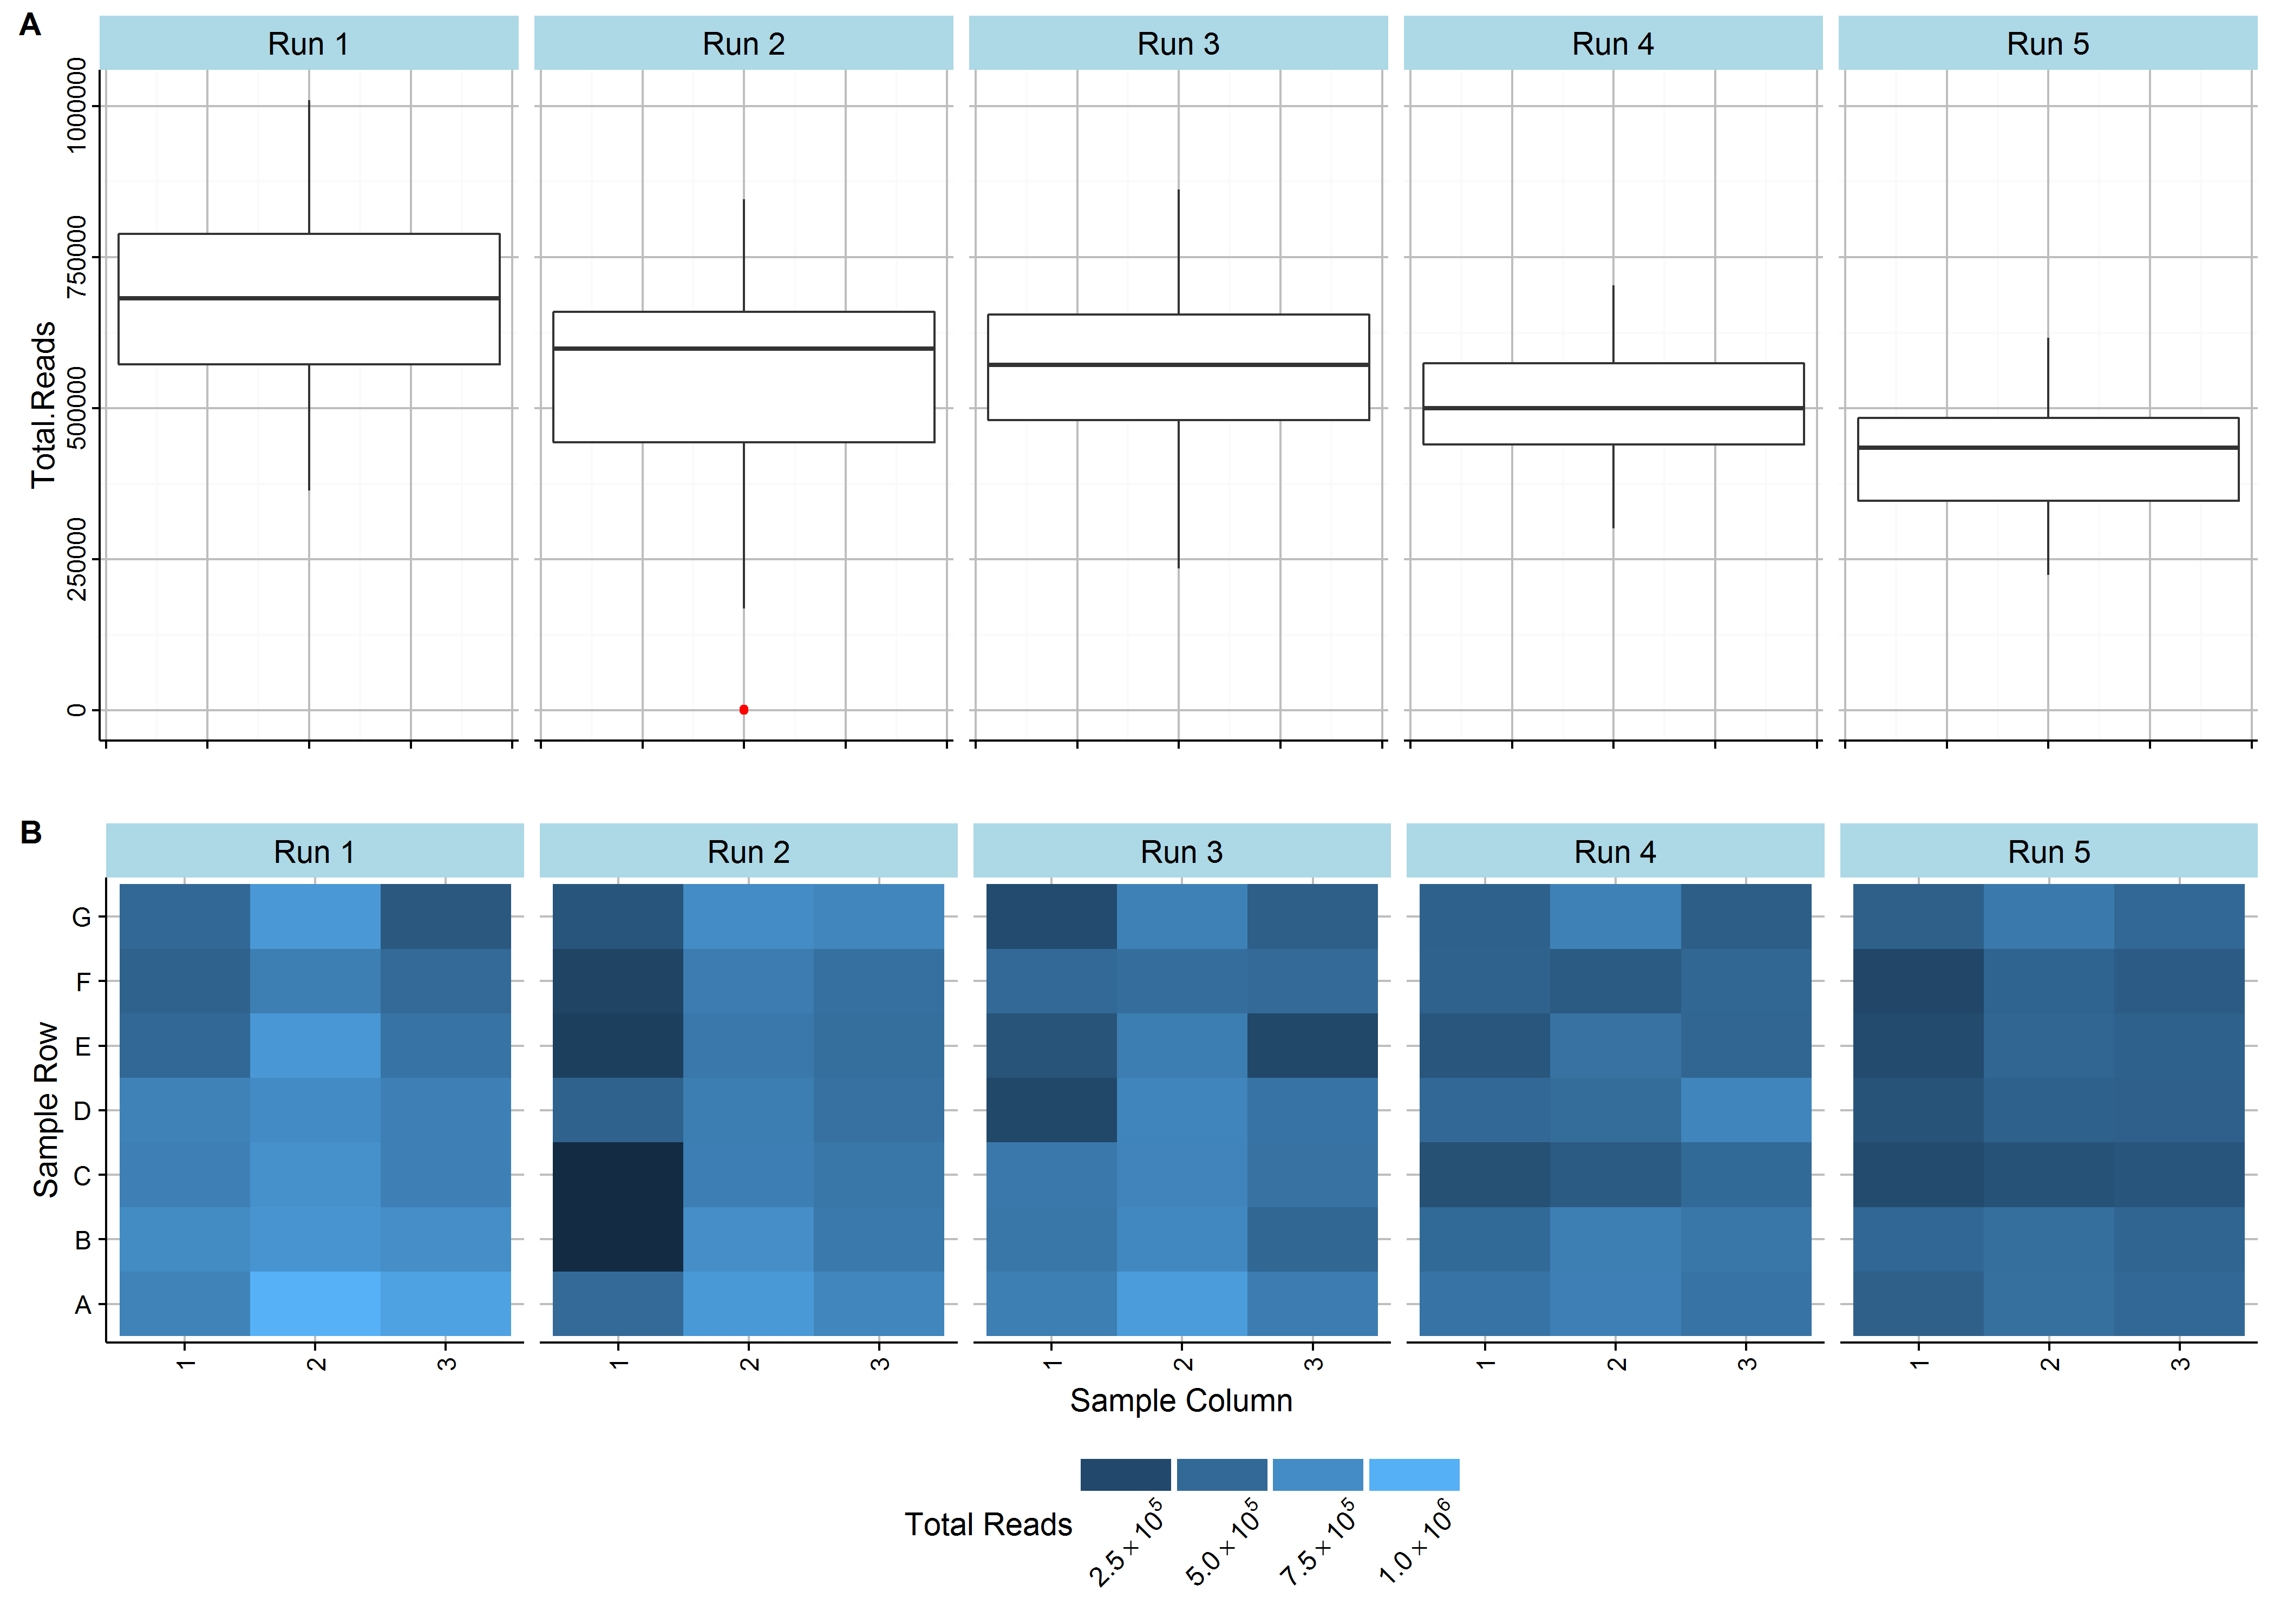
\includegraphics[scale=.5]{./Figures/IO_Repro_Combined_RawTotals}
\caption{A) Distributions of total reads allocated to each sample in five runs on an Illumina Mi-Seq sequencer. Only one sample is identified as a problematic sample. B) Heat-maps showing the relative totals for each sample within each run.  The darker heat-maps for runs 4 and 5 reflect the generally lower number of total reads in those sequencing runs as compared to runs 1 and 2.  This is caused by normal variation in the number of reads available in a sequencing run.}
\label{totalFig}
\end{figure}
 
\begin{figure}
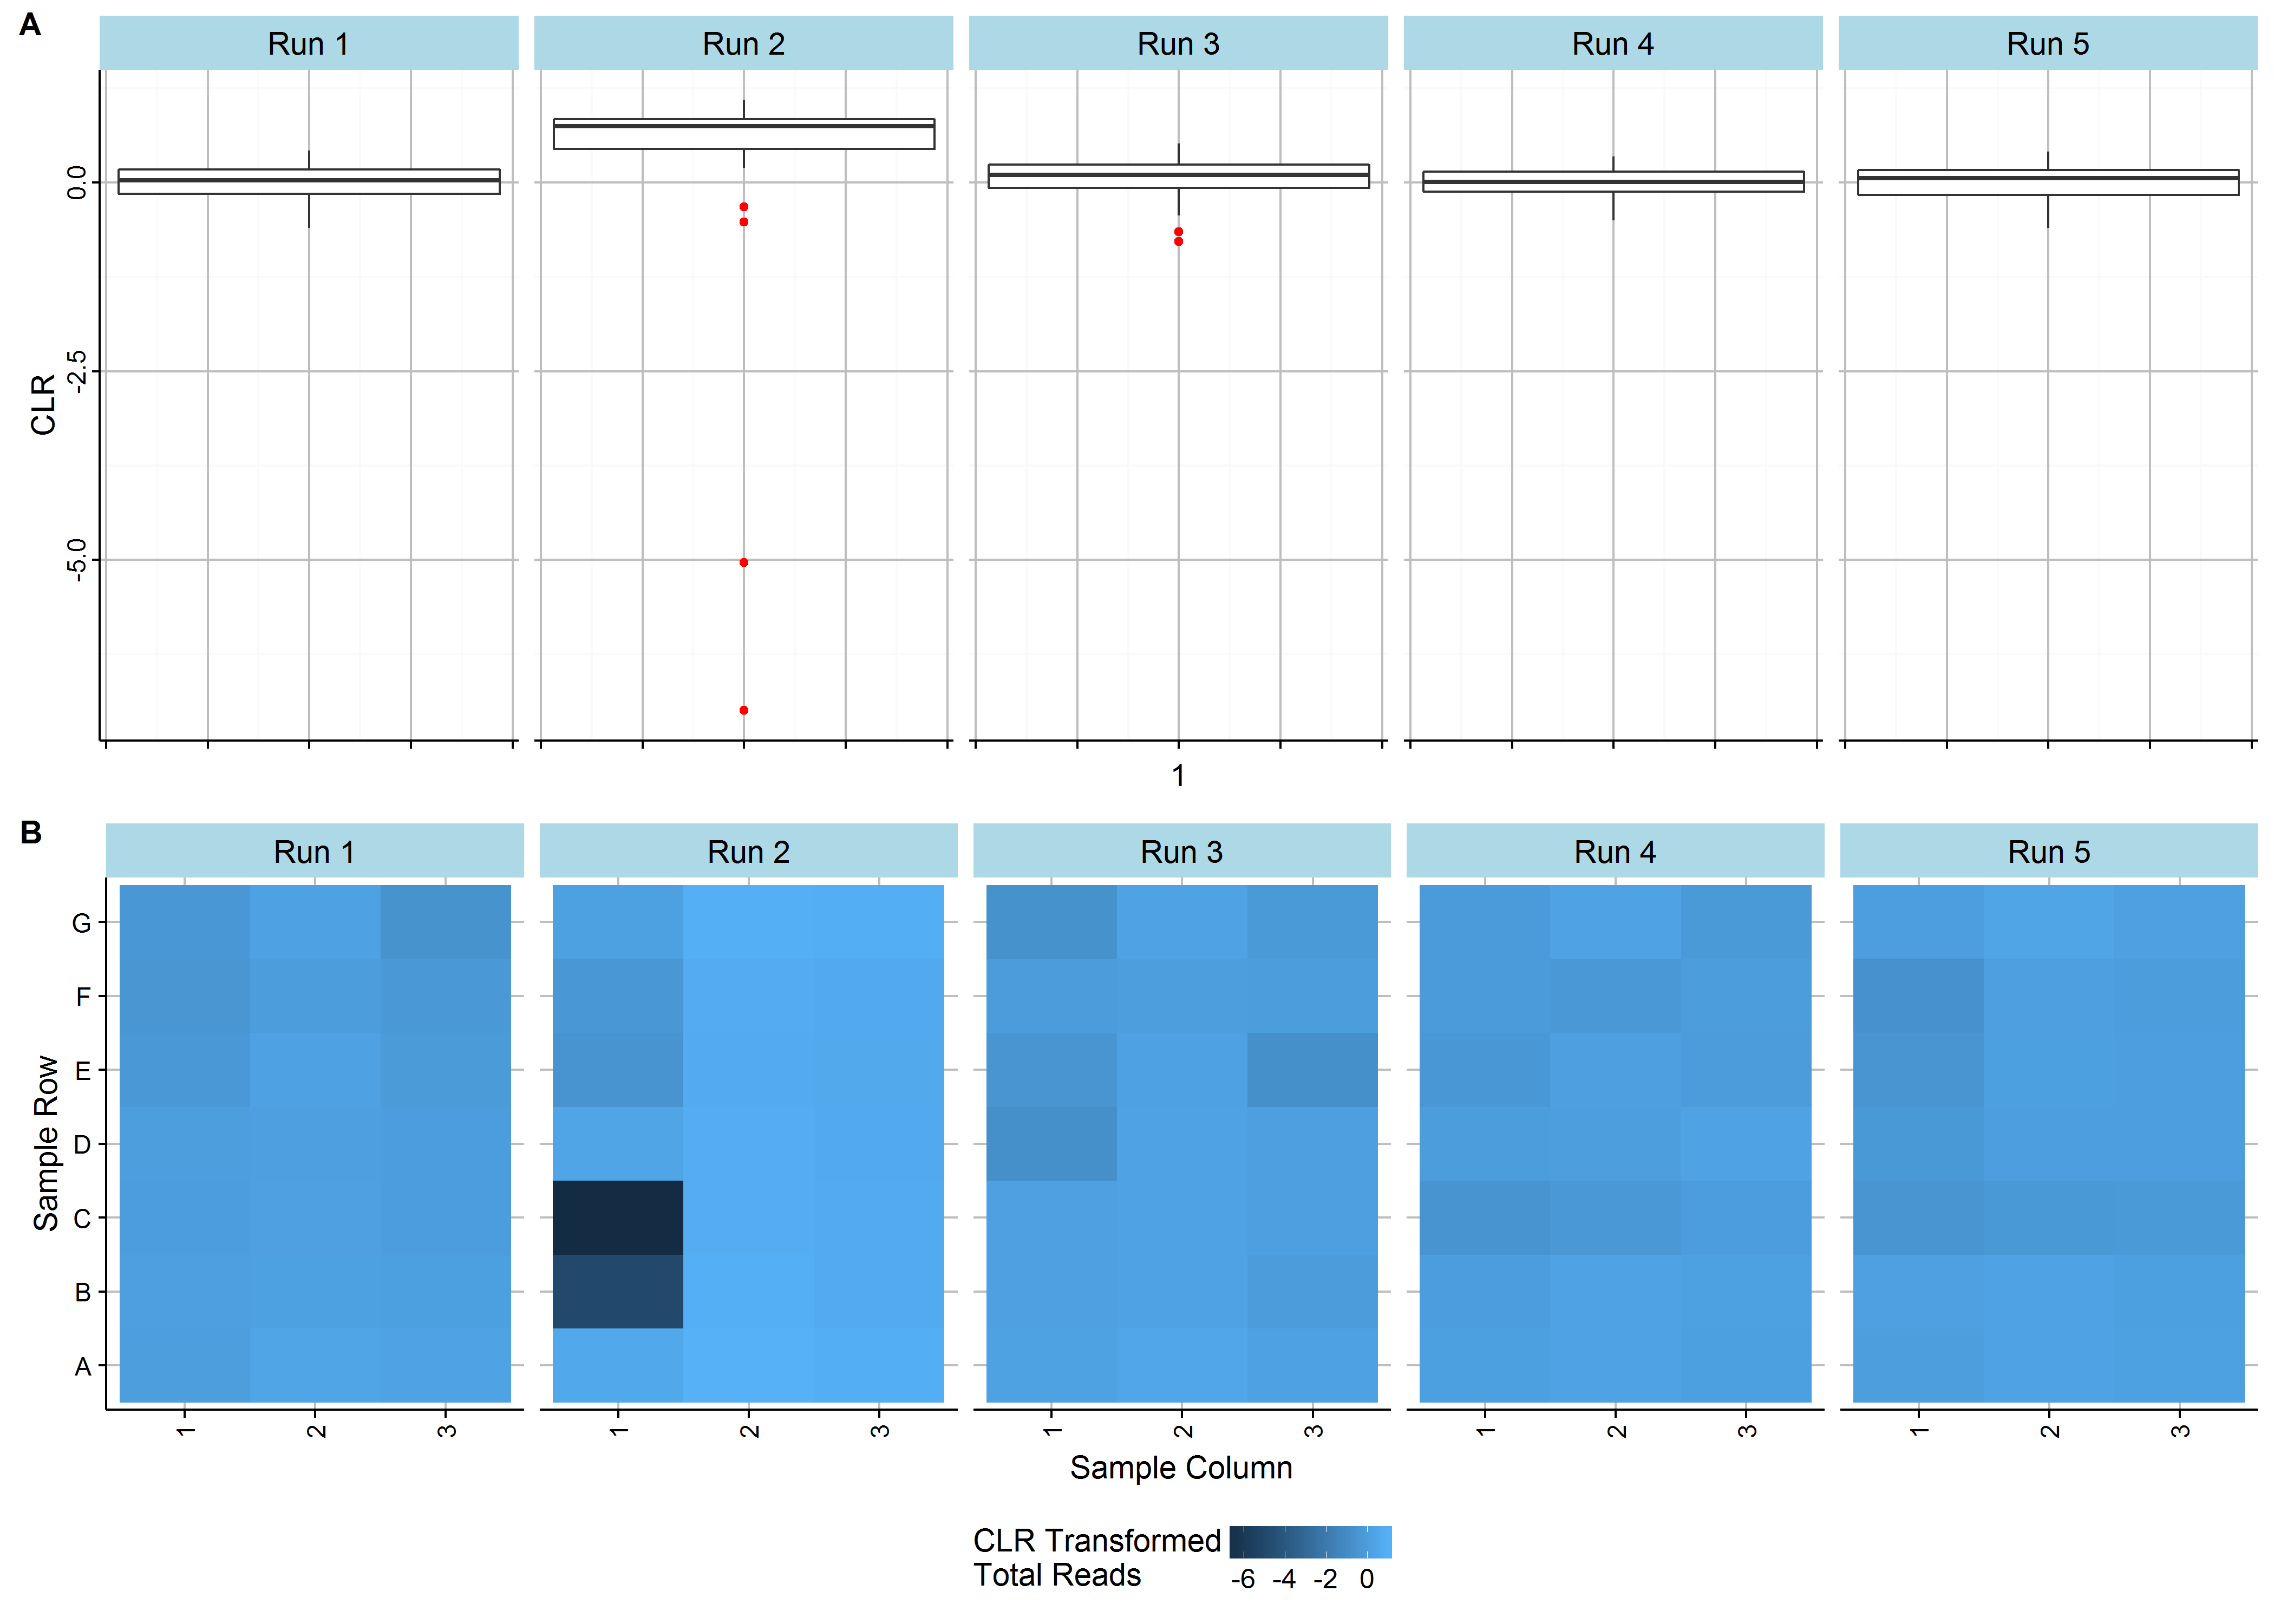
\includegraphics[scale=.5]{./Figures/IO_Repro_Combined_CLR}
\caption{A) Distributions of CLR transformed total reads allocated to each sample in 5 runs on an Illumina Mi-Seq sequencer. After CLR transformation, six samples are identified as a problematic. B) Heat-maps showing the relative CLR transformed totals for each sample within each run.}
\label{clrFig}
\end{figure}

\FloatBarrier
\section{Testing for Compositional Invariance}

%Traditional testing for CI has several problems
%   - Choice of denominator will impact the number of probes which exhibit CI violations
%   - Increases in variance associated with low reads will make it hard to identify CI violations
%   - How much CI violation is too much?  100 betas != 0?  200? 1000?



Normalization and standardization methods for RNA-Seq generally assume that the total number of reads assigned to a sample does not affect the observed relative frequencies of probes within an assay.  For example, implicit in the CPM transformation is the idea that if you re-scale the counts (by dividing by the total for each sample) then the resulting counts are comparable and any differences are due to underlying differences in expression.  Other methods which apply a scaling factor to each sample, such as TMM or Quantile normalization, also rely on this assumption.  In the parlance of compositional data these methods assume \emph{compositional invariance} (CI), i.e. the underlying composition is statistically independent of the total size of the composition (the total counts for a sample, $t$).

Compositional invariance is an important assumption for RNA-Seq data because it enables the comparison of samples with differing read depths.  However, it is well documented that the quality of RNA-Seq depends on the read depth, where higher read-depth is associated with higher quality data~\cite{Tarazona2011,Sims2014}. Read depth may affect the measurement of relative abundances for the target RNA sequences as some targets may receive proportionally more reads as the read depth increases.  This would be a direct violation of CI and could lead to seemingly differential expression between samples with different read depths, even after normalization.  Another form of CI violation, that is perhaps more likely in RNA-Seq experiments, is the dependence between the variance of read counts and the read depth.


Aitchison~\cite{Aitchison1986} outlined a simple model for testing compositional covariance using the ALR transformation,  

\begin{equation}
\left[y_1 \ldots y_d \right] = 
\left[
\begin{array}{cc}
1 & t
\end{array}
\right]
\left[
\begin{array}{ccc}
\alpha_1 & \cdots & \alpha_d\\
\beta_1 & \cdots & \beta_d
\end{array}
\right] 
+
\left[e_1 \ldots e_d \right],
\label{matrixModel}
\end{equation}

where $y_1 \ldots y_d$ are the $d$ ALR transformed components, $t$ is the vector of sample total aligned reads, $\alpha_1 \ldots \alpha_d$ are the probe specific log-ratio intercepts, and $\beta_1 \ldots \beta_d$ are the coefficients relating the the total aligned reads to the relative expression of the probe.  A test for compositional invariance for the experiment then becomes a test of the null hypothesis, $H_o: \beta_1 = \cdots = \beta_d = 0$. This test can be re-parameterized to test for dependence between the variance and total aligned reads as well.


Unfortunately, the small sample sizes and large number of probes typically associated with RNA-Seq experiments complicates the application of Aitchison's model.  
We propose an alternative visualization for simultaneously detecting both violations of compositional invariance described above. We use the multivariate Aitchison distance (\ref{aitchdist2}) between all pairs of samples in a heat-map with the samples ordered by total aligned reads.  If CI is violated we expect pairs samples with similar total aligned reads will have smaller scalar distances than those with large differences in total aligned reads.  This will result in visual clustering around the 45 degree axis. If the variance depends on the total aligned reads, we expect the scalar distance between sample pairs to decrease with increasing read depth resulting in a visual gradient in the distance heat map.  To reduce the visual noise associated with outlier samples in the heat-map we also provide a dot-plot of the distance between each CLR transformed sample and the compositional center of the samples in the top quartile of total reads. We also provide a least-squares estimated regression line for the relationship between the distance metrics and the order of the samples based on total aligned reads.

We demonstrate this visualization with two sets of miRNA samples (Fig.~\ref{miComp}) and two sets of mRNA samples(Fig.~\ref{celComp}).  The miRNA samples are composed of 40 technical replicates each of (1) plasma samples and (2) brain samples.  In the miRNA data there is a clear gradient along the 45 degree axis for the plasma samples (Fig.~\ref{miComp}.A).  This indicates a dependence between the total aligned reads and the variance of the samples (as indicated by the increasing multivariate distance between replicates as the total aligned reads decreases).  In contrast, there is no clear gradient in the brain samples (Fig.~\ref{miComp}.B).  The mRNA samples are composed of (A) 16 technical replicates of diseased pancreas tissue and (B) 16 technical replicates of normal pancreas tissue.  In the diseased pancreas samples there is a clear gradient with low total aligned read samples more distant from samples with greater total aligned reads (Fig.~\ref{celComp}.1).  This indicates that the composition is dependent on the total aligned reads, a violation of compositional invariance for these samples.  In contrast, the normal pancreas samples show no such pattern related to total aligned reads (Fig.~\ref{celComp}.2).

\begin{figure}
\centering
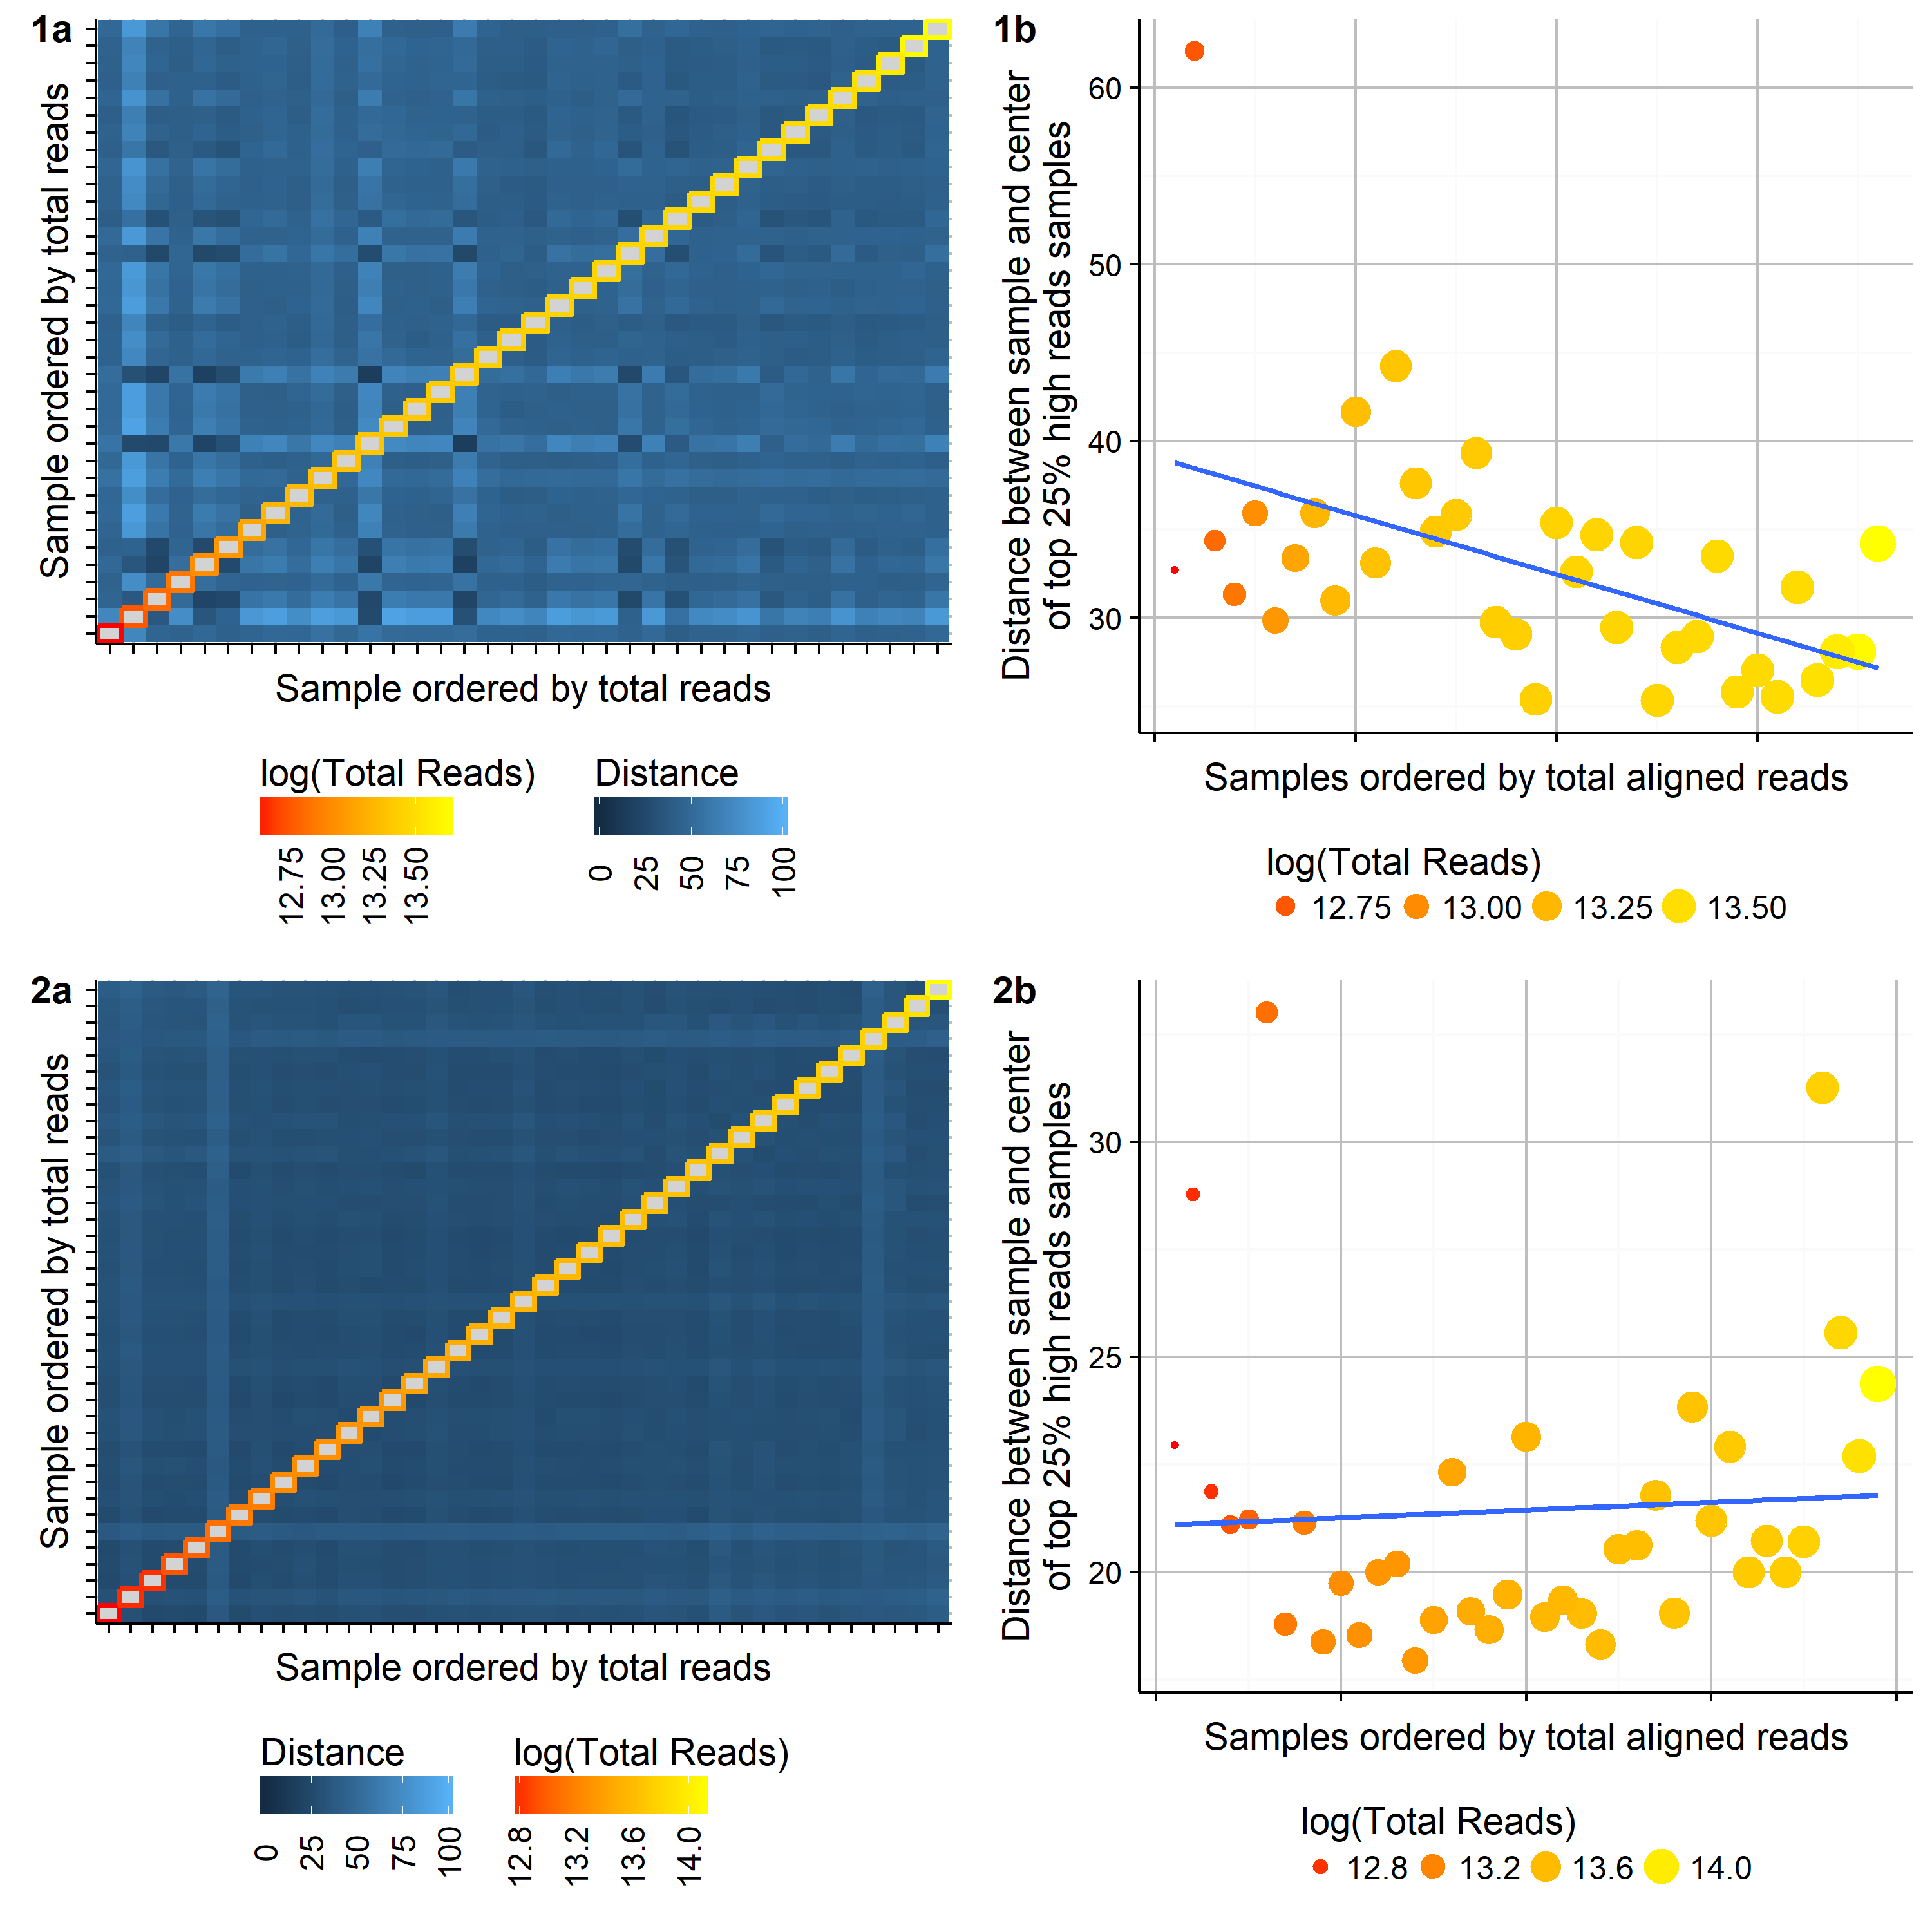
\includegraphics[scale=0.6]{./Figures/CompInvPlots_miRNA}
\label{miComp}
\caption{Two sets of miRNA samples with samples in (1.) showing a violation of compositional invariance and (2) showing compositional invariance.}
\end{figure}


\begin{figure}
\centering
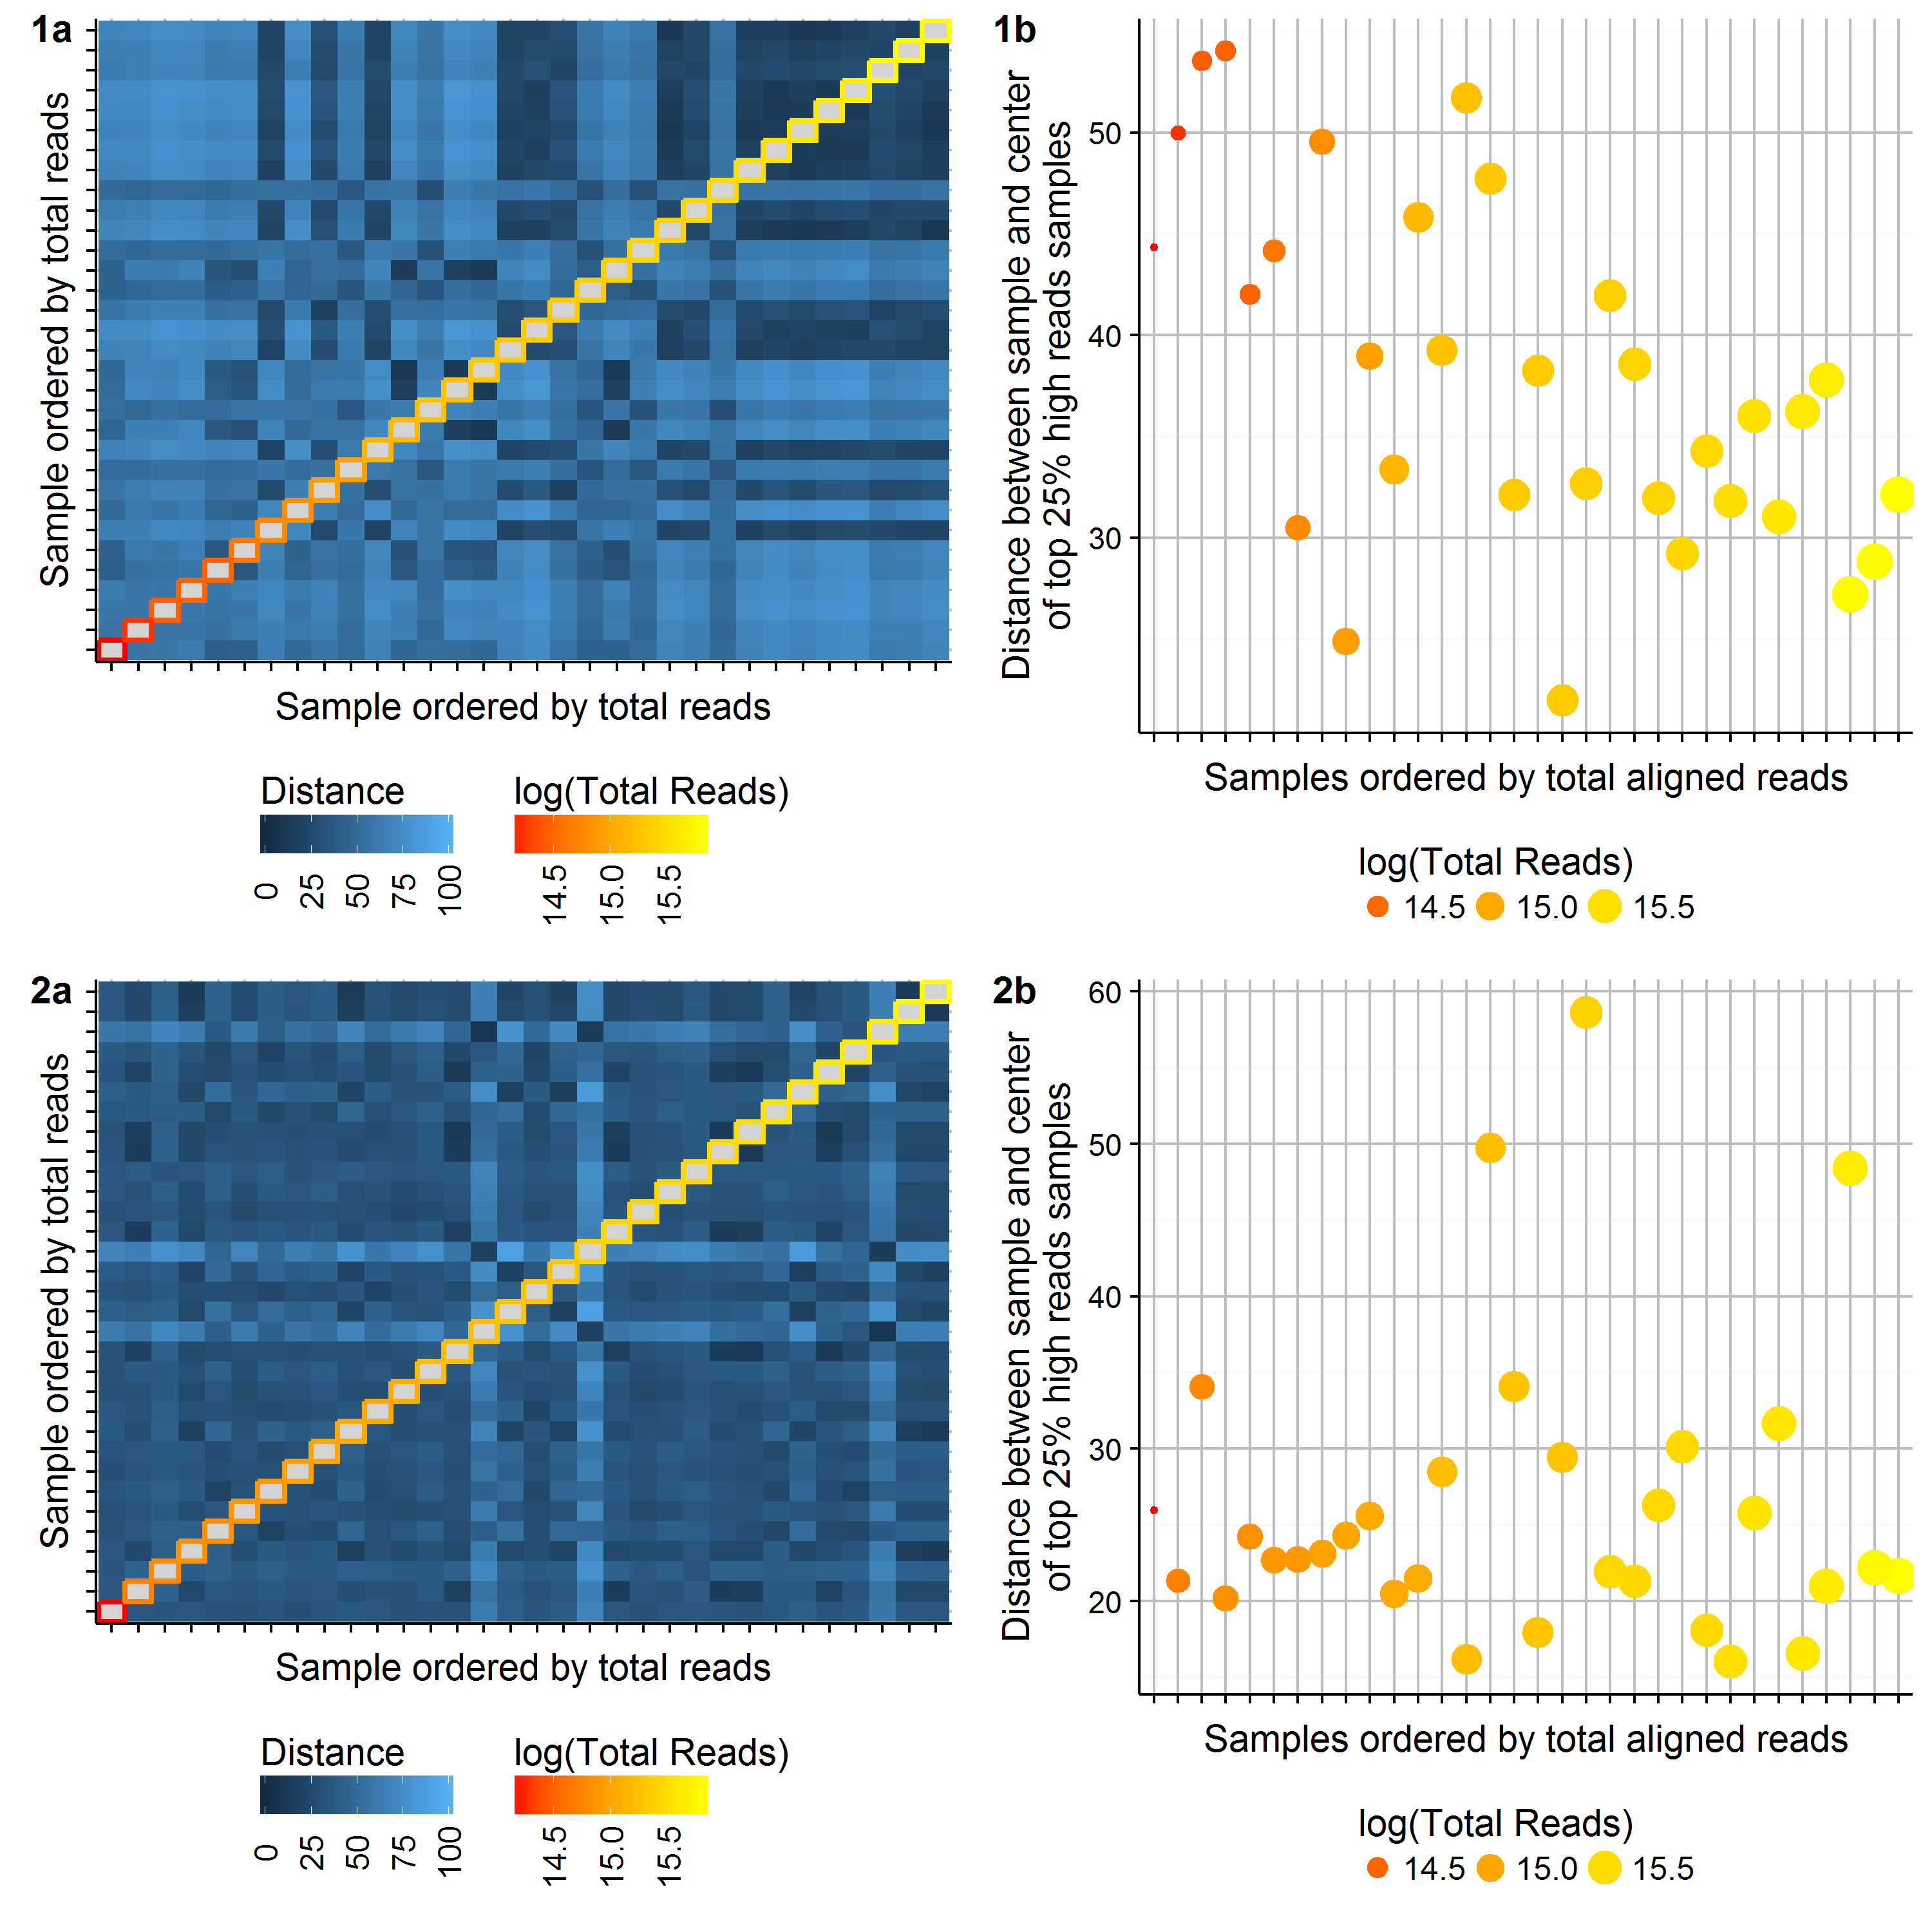
\includegraphics[scale=0.6]{./Figures/CompInvPlots_Celgene}
\label{celComp}
\caption{Two sets of mRNA samples with samples in (1.) showing a violation of compositional invariance and (2) showing compositional invariance.}
\end{figure}

\FloatBarrier
\section{Batch Effects and Normalization}

Batch effects arising from differing laboratory conditions or operator differences have been identified as a problem in high-throughput measurement systems~\cite{leek2010, chen2011}.  Identifying and controlling for batch effects is a critical step in the transition of RNA-Seq from the lab to the clinic.  Batch effects are typically identified with a hierarchical clustering (HC) method or principal components analysis (PCA).  For both methods, the multivariate distance between the samples is visualized, either in a biplot~\cite{Aitchison2002} for PCA or a dendrogram for HC, to check for the existence of clusters of samples related to batch.
The compositional nature of RNA-Seq data has important implications for the detection of batch effects due to the incompatibility with standard measures of distance between compositions as noted above~\cite{Aitchison1986,Martin-Fernandez1998}.

Principle components analysis is sensitive to differences in scale (total number of reads) among the variables, failure to remove these difference can mask potential batch effects and leave unwanted technical variation in the data.  As noted above, most normalization methods use a scaling factor calculated for each sample to re-scale the read count for each gene within the sample~\cite{Dillies2013}.  The CLR transformation can similarly be viewed as a scaling normalization (with the scale factor chosen as the inverse of the geometric mean $1/g(x)$).  Unlike other normalization methods, the CLR transformation has the added benefit of being applied at the individual sample level, not experiment wise like quantile or median normalization~\cite{Bolstad2003}, and requires no assumptions about differential expression among samples like quantile or median ratio normalization~\cite{Robinson2010,Anders2010}.  This makes it particularly well suited for the clinic where there are generally no reference samples for normalization.  Most importantly, CLR transformation allows the use of Euclidean geometry, such as Euclidean or Mahalanobis distance, so that standard PCA or HC applied to transformed samples can be interpreted under theory of linear models ~\cite{Aitchison2002} .

We use a compositional biplot to detect batch effects using 120 technical replicates of three sample types: brain, plasma, and FFPE.  Samples were prepared using the EdgeSeq Whole Transcriptome miRNA assay which measures 2,280 targets including 11 control probes and 2,269 unique miRNA probes.  All sequencing was performed on an Illumina Mi-seq$^{(tm)}$ sequencer.  First, we obtain linear components using PCA on log-transformed and CLR transformed data and then create biplots of the first two principle components for each transformed data set (Fig.~\ref{rawPCA}).  The differences between the three samples types (brain, plasma, and FFPE) dominate the first two principle components for both data sets.  However, the CLR transformed data provides tighter clusters, relative to the distance between the clusters, than the log-transformed raw data.  There is also a single FFPE sample which is closer to the brain samples than the other samples.  It is worth noting that this sample would have been removed using our proposed quality control metric.  Since the sample type differences overwhelm the potential batch effects we performed a second PCA on only the brain samples for both transformed data sets (Fig.~\ref{rawPCAbrain}).  Both biplots exhibit clustering by batch but the CLR transformed data shows better separation between the batches. 

\begin{figure}
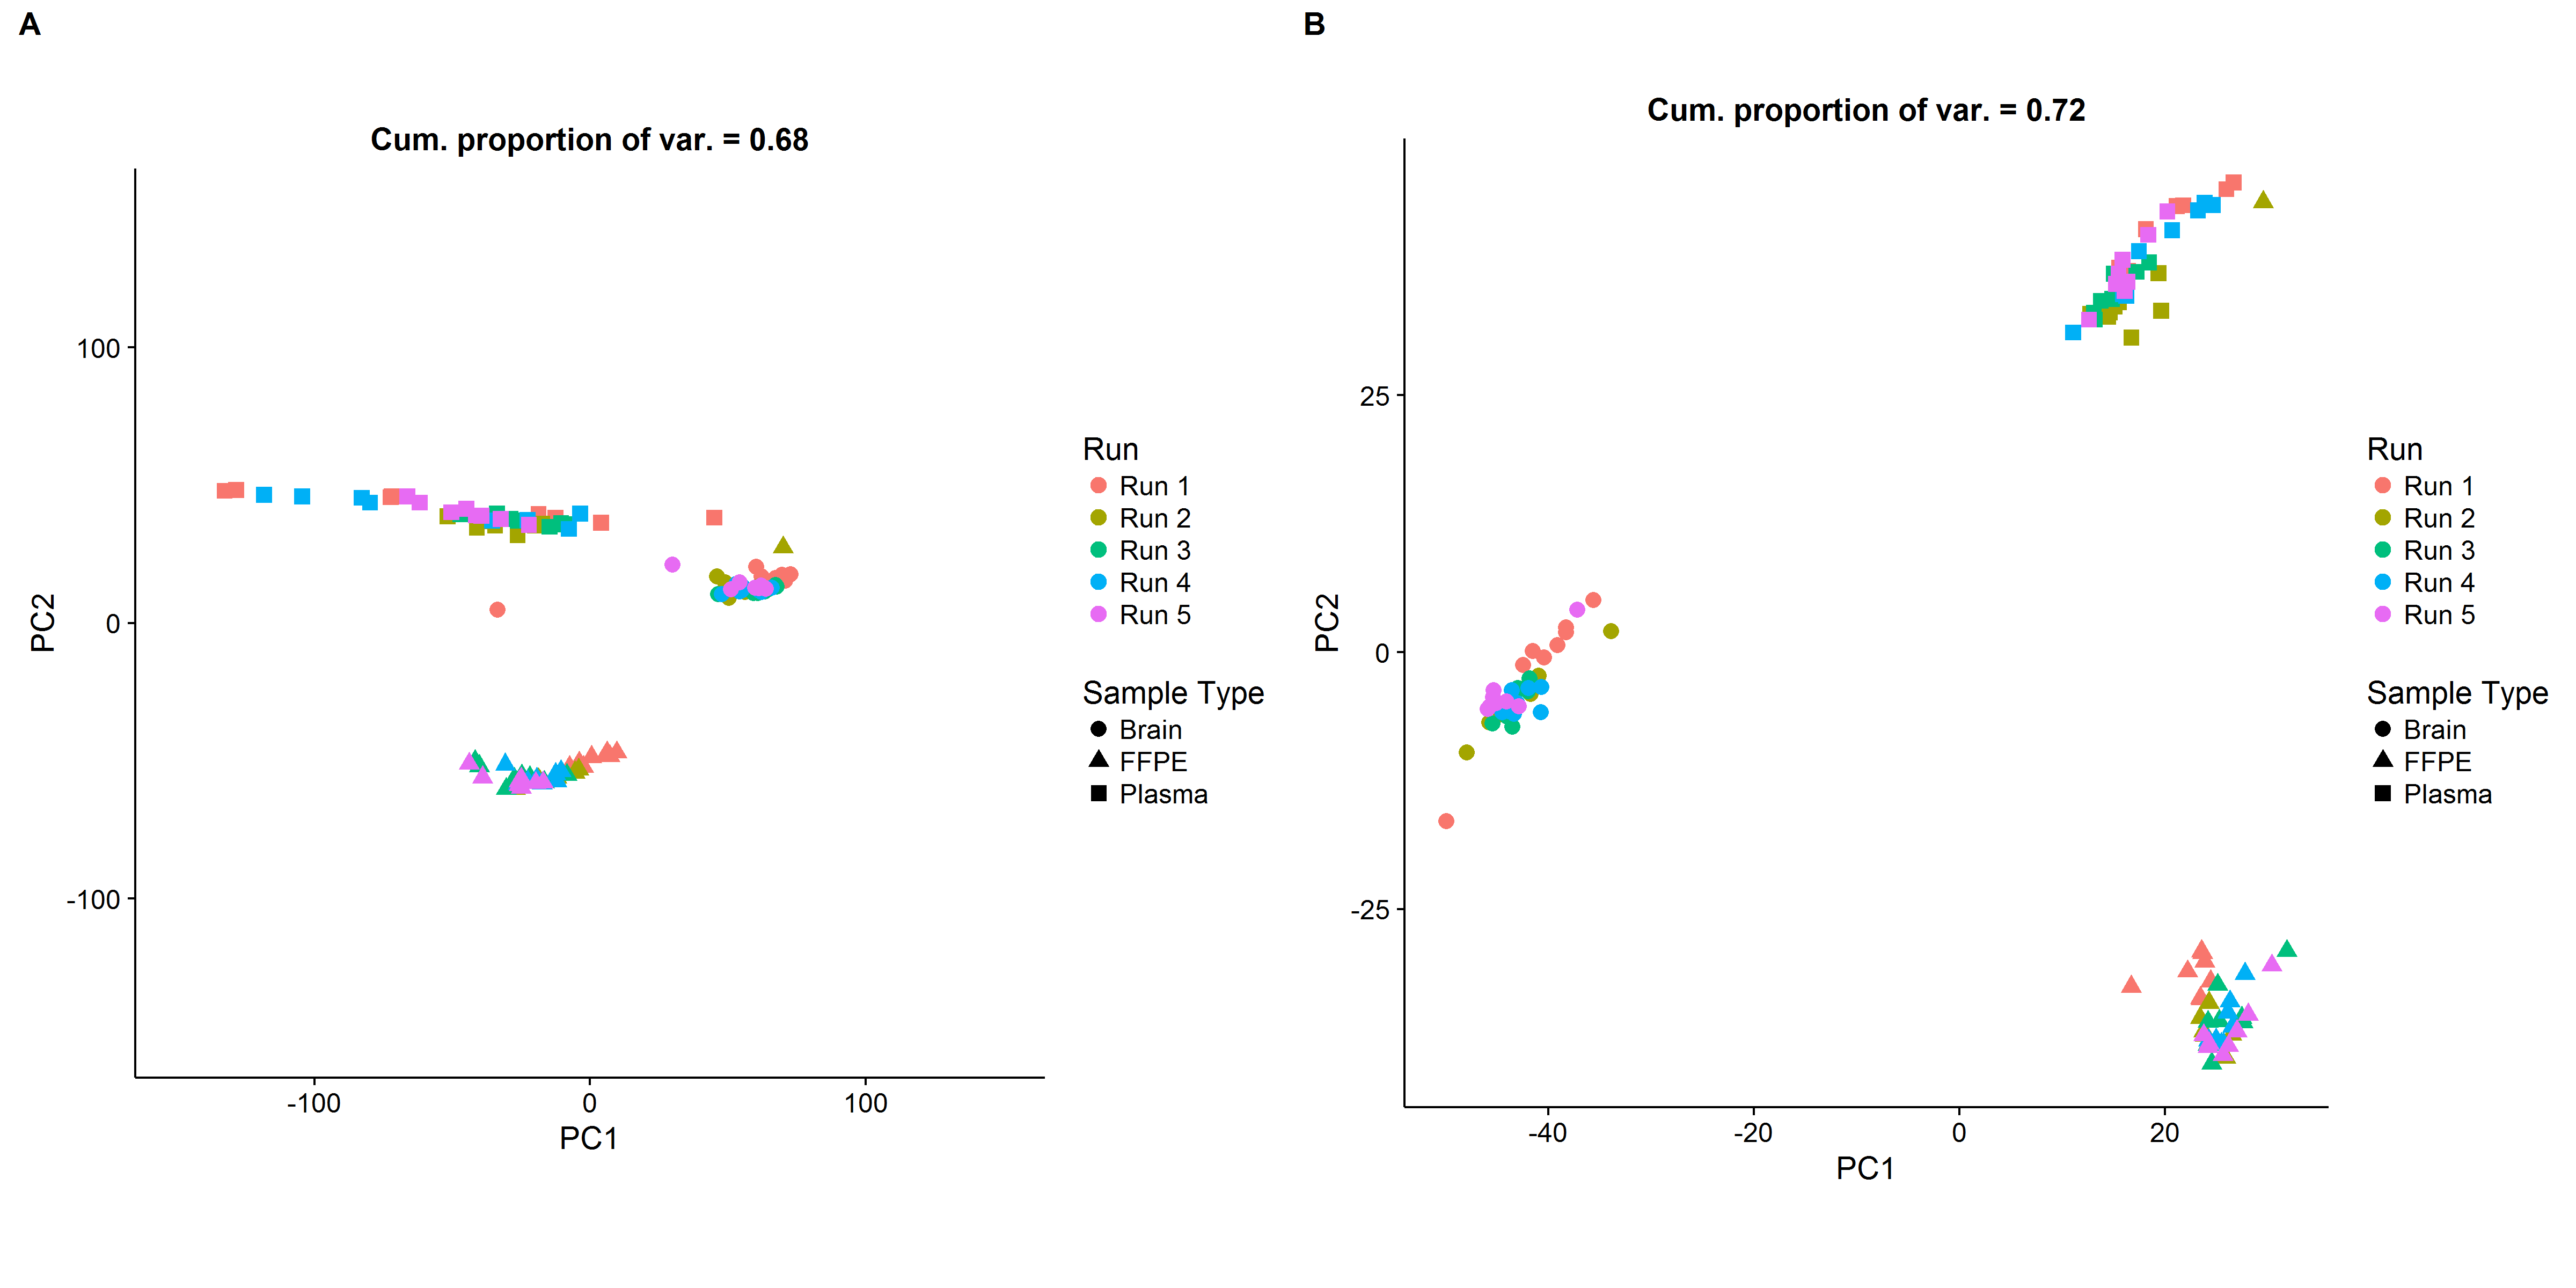
\includegraphics[scale=0.4]{./Figures/IO_PCA_2plot}
\label{rawPCA}
\caption{Principle component analysis of A) log-transformed and B) CLR-transformed read count data.  The differences between sample types is much greater than the batch effects in both transformation.  The CLR transformation results in tighter sample type clusters resulting from less variation along the first principle component. }
\end{figure}



\begin{figure}
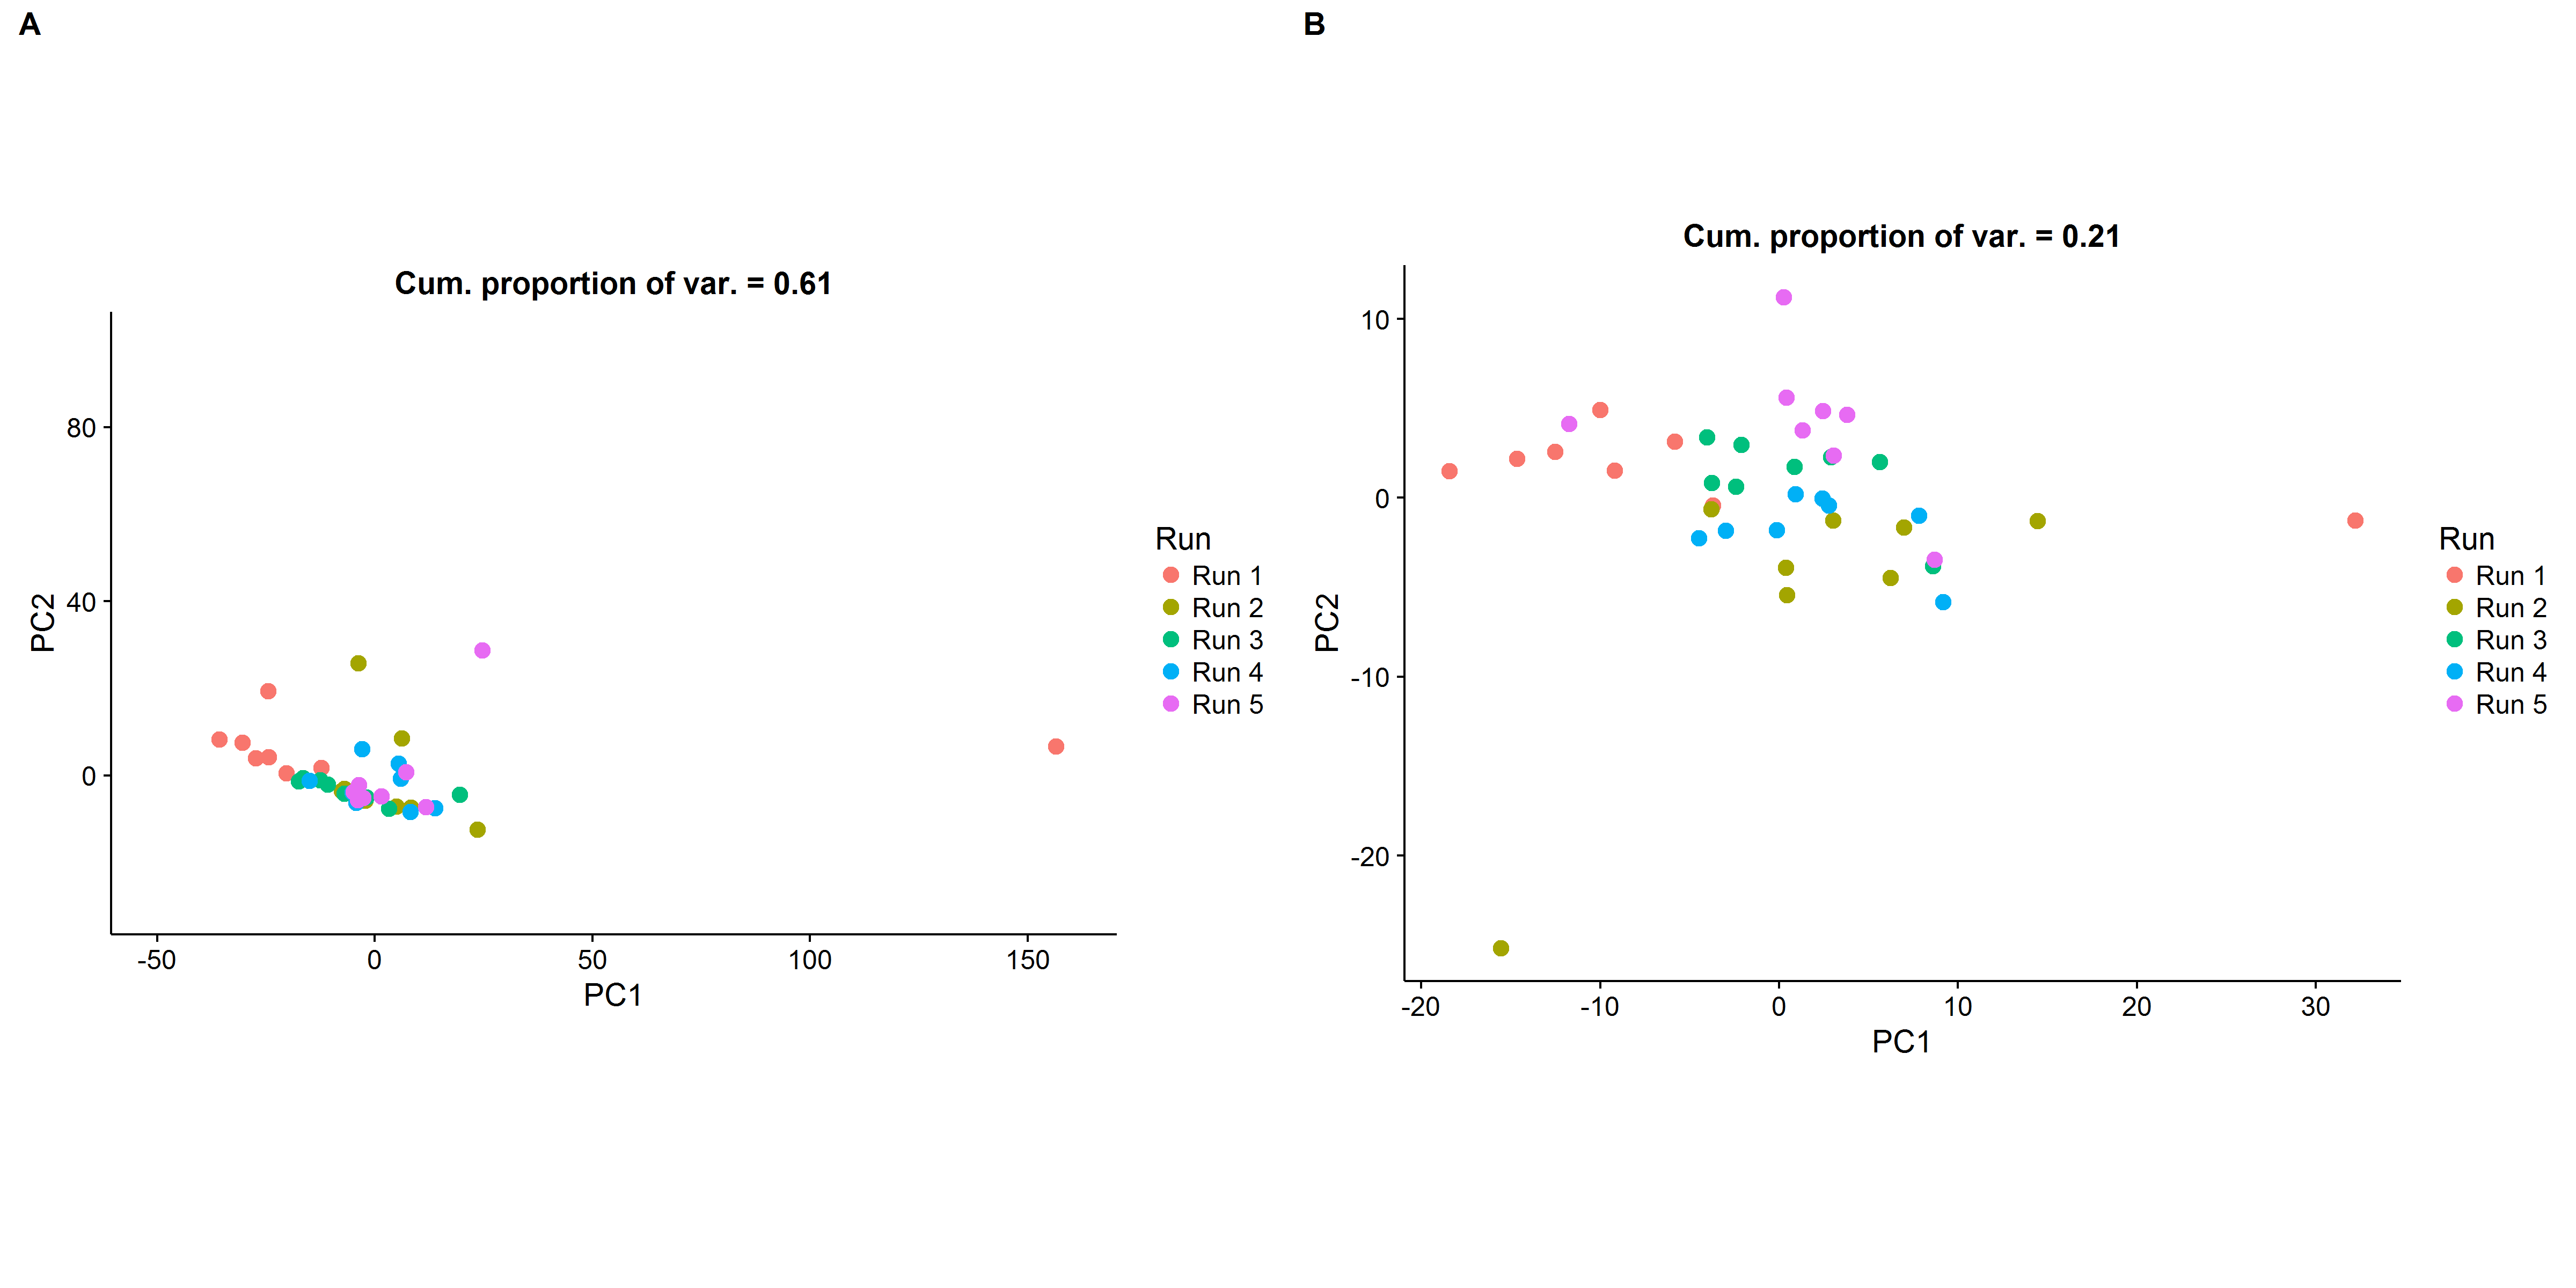
\includegraphics[scale=0.4]{./Figures/IO_PCA_Brain_logRaw_CLR}
\label{rawPCAbrain}
\caption{Principle component analysis of only brain samples from A) log-transformed and B) CLR-transformed read count data. The batch effects are more easily identified in the CLR transformed data.}
\end{figure}



\FloatBarrier
\section{Discussion}

Our fractional read allocation metric can identify problematic samples which arise from multiple failure modes, e.g. a low quality sample or a sequencing problem.  However, it is conceivable that a sample might have an unusually low (or high) number of reads and still provide quality information.  In certain experimental designs one might be able to further evaluate these samples with a PCA biplot on the CLR transformed data. In our PCA analysis we identified a FFPE sample which would have failed our quality control and was clearly very different from the other technical replicates.  However, if this sample had remained quite similar to the other FFPE replicates this would have provided information that the sample may still be valuable.  In this way, the quality control metric and PCA biplot can be used in tandem to provide additional information about the quality of a sample.\\

The compositional invariance visualization is a logical extension of the sample quality control metric since the assumption of the sample quality control is that the total number of aligned reads is related to the proportional allocation of reads within the sample.  As noted above samples which violate the compositional invariance property may still contain valuable information.  The identification of compositional invariance violations allows the investigator to account for the dependency between the total aligned reads and the relative abundance of transcripts within the samples when modelling.

The principal components analysis biplot is a well know dimension reduction visualization.  For the current data the dimension is reduced from 2,280 probes to 2 principle components.  The utility of the data reduction, including the quality of the approximation of the multivariate distance between the samples, is proportional to the amount of variance explained by these two principle components. In our data the first two principle components explain 72 and 21 percent of the variation, respectively.  The analysis with the lowest percent of variation explained by the first 2 components is of the CLR-transformed brain samples.  Surprisingly, batch effects are still visible in this plot, in which case they can be removed~\cite{Luo2010}.  

As RNA-Seq makes the transition from the research laboratory to the clinic there is a need for robust quality control metrics.  The realization that RNA-Seq data are compositional opens the door to the existing body of theory and methods developed by Atichison and others.  We show that the properties of compositional data can be leveraged to develop new metrics and enhance existing methods.\\



\newpage
%\printbibliography
\bibliographystyle{spmpsci} 
\bibliography{proportionality}















\end{document}

